\documentclass[a4paper,12pt,twoside]{book}

\usepackage{polski}
\usepackage{fancyhdr} %naglowek i stopka
\usepackage[cp1250]{inputenc} %polskie znaki
\usepackage{graphicx} %wstawianie grafili
\usepackage{anysize} % do margines?w
\usepackage{indentfirst} %polskie "normy" akapitow
\usepackage{textcomp} %nazwisko czecha
\usepackage{afterpage}
\usepackage{amsthm}
\usepackage{float}

\pagestyle{fancy} 	
\fancyhead{} \fancyfoot{} 

\renewcommand{\chaptermark}[1]{\markboth{#1}{}}
\renewcommand{\sectionmark}[1]{\markright{\thesection\ #1}}

\fancyhead[RE,LO]{\normalfont \thepage}
\fancyhead[RO]{\normalfont \rightmark}
\fancyhead[LE]{\normalfont \leftmark}

\fancypagestyle{plain}{\fancyhead{}\renewcommand{\headrulewidth}{0pt}} 

\marginsize{3,5cm}{2,5cm}{2,5cm}{2,5cm}


\begin{document}
\tableofcontents
\chapter{Wst�p} \label{wstep} 
Celem projektu in�ynierskiego jest budowa  autonomicznego pojazdu mobilnego przypominaj�cego czo�g. Temat pracy jest bardzo otwarty, co pozwala na du�� swobod� dotycz�c� wyboru za�o�e� konstrukcyjnych. Robot zostanie wyposa�ony w obrotow� wie�yczk� znajduj�c� si� na korpusie pojazdu oraz zamocowanym do niej ,,dzia�em" mog�cym zmienia� swoje po�o�ene. Urz�dzenie w spos�b autonomiczny stara si� zlokalizowa� cel oraz okre�li� jego po�o�enie wzgl�dem samego siebie. W ramach projektu nale�y: zbudowa� robota, wykona� projekt elektroniki, zaimplementowa� algorytm steruj�cy robotem, przeprowadzi� niezb�dne testy dzia�ania systemu oraz przygotowa� dokumentacj� techniczn�.

Koncepcja inteligentnych robot�w bojowych znajduje si� w kr�gu zainteresowa� s�u�b specjalnych takich jak wojsko czy policja. Pozwalaj� one przeprowadza� wiele niebezpiecznych operacji bez nara�ania �ycia za�ogi. Podczas prowadzenia wojen najwi�kszy nacisk k�adzie si� na ochron� �o�nie�y, z tego wzgl�du �e wyszkolenie i zaadaptowanie nowej osoby na miejsce do�wiadczonej i wykwalifikowanej jednostki zajmuje zbyt wiele czasu oraz jest zanadto kosztowne. 

Autonomiczne pojazdy bojowe mog� dociera� do miejsc, kt�re s� niedost�pne dla ludzi oraz zdalnie sterowanych robot�w. Cz�sto posy�ane s� w miejsca, w kt�rych komunikacja radiowa czy przewodowa z robotem jest niemo�liwa b�d� niestabilna, np. podczas prac prowadzonych w jaskiniach, zawalonych budynkach, tunelach b�d� pod wod�. Nawet sterowane przez cz�owieka maszyny, wykonuj�ce zadania w trudnych warunkach, powinny mie� zaimplenetowane proste algorytmy, kt�re przypadku utraty ��czono�ci, pozwalaj� na zachowanie aktualnej pozycji i podj�cie pr�b wznowienia komunikacji.

Pojazdy te bior� czynny udzia� w licznych badaniach naukowych oraz operacjach ratunkowych - nie tylko wojskowych, ale tak�e medycznych. Zadania, kt�re s� przed nimi postawione s� niejednokrotnie bardzo odpowiedzialne, gdy� to od nich mo�e zale�e� ludzkie �ycie. W zwi�zku z tym nie mog� pope�nia� b��d�w zwi�zanych z b��dn� interpretacj� odebranych z czujnik�w informacji. Podczas tworzenia projektu bardzo du�y nacisk b�dzie na�o�ony na algorytm przetwarzanie obrazu otoczenia aby mo�liwie skutecznie oraz jednoznacznie rozpozna� cel.

Wyb�r tego tematu podyktowany by� przede wszystkim ch�ci� zbudowania robota. Moim zdaniem jest to zwie�czenie ca�ej zdobytej podczas trwania studi�w wiedzy. Proces budowy autonomicznego pojazdu sk�ad�cy si� zar�wno z zaprojektowania cz�ci mechanicznej jak i programowej, jest bardzo wymagajacy i z�o�ony. Wymaga on od konstruktowa nie tylko wiedzy teoretycznej dotycz�cej zasady budowy i dzia�nia poszczeg�lnych podzespo��w, ale tak�e opanowania technik zwi�zanych z sterowaniem oraz komunikacj� pomi�dzy r�ego typu urz�dzeniami. Realizacja tego projektu pozwoli na sprz�enie wiedzy teortycznej ze �wiatem rzeczywistym oraz ocene skuteczno�ci zastosowanych rozwi�za�.

Autonomiczne roboty mobilne najcz�ciej poruszaj� si� w nie do ko�ca znanym im �rodowisku. Co za tym idzie - musz� by� wyposa�one w system nawigacyjny, przez kt�ry rozumiany jest zesp� czujnik�w pe�ni�cych funkcj� sprz�enia zwrotnego z otaczaj�cego pojazd �wiata. W naszym przypadku system g��wnie opiera� si� b�dzie o mikrokomputer wyposa�ony w kamer� video, kt�ry dodatkowo b�dzie wspierany kilkoma czujnikami odleg�o�ci. Ich zadaniem b�dzie przede wszystkim wykrycie mo�liwych kolizji z przedmiotami znajduj�cymi si� bezpo�rednio przed robotem. Projekt oparty b�dzie o tzw. system wbudowany, czyli kompaktow�, multimedialn� jednostk� obliczeniow� wykorzystywan� do realizacji specjalnych funkcji takich jak sterowanie prac� silnika czy analiza danych. Systemy wbudowane s� (najcz�ciej) na sta�e po��czone z elementami wykonawczymi oraz pomiarowymi. Najwa�niejsz� funkcj� czo�gu b�dzie przetwarzanie oraz analizowanie obraz�w w czasie rzeczywistym, co wymaga stosunkowo du�ej pami�ci oraz mocy obliczeniowej. Powy�sze wymagania pozwoli�y wybra� platform�, na kt�rej zrealizowany b�dzie projekt, mianowicie \textit{Raspberry Pi} wraz z dedykowan� kamer� \textit{Raspberry Pi Camera Board}. 
Wyb�r modelu zawieszenia dla czo�gu jest jednoznaczny - g�sienice. Rozwi�zanie tego typu jest najcz�ciej spotykanym systemem jezdnym pojazd�w wojskowych. Roboty bojowe cz�sto zmuszone s� porusza� si� w bardzo zr�nicowanym i nieprzyjaznym �rodowisku. Stawia to przed uk�adem zawieszenia wiele wyzwa�.  G�sienice - dzi�ki r�wnomiernemu roz�o�eniu ci�aru (wiele pasywnych osi), du�ej powierzchni styku z pod�o�em, prostocie sterowania oraz trwa�o�ci s� niew�tpliwie najlepszym rozwi�zaniem w tej dziedzinie.


\namedchapter[Adam Zieliński]{Rys historyczny}
Słowo ,,robot" wywodzi się z języka czeskiego, gdzie oznacza ciężką pracę. 
Według słownika języka polskiego słowo to oznacza urządzenie zastępujące człowieka przy wykonywaniu niektórych czynności\cite{SJP}. Po raz pierwszy, w tym kontekście, zostało ono użyte w 1920 r. przez czeskiego pisarza Karela \newtie{C}apka w komedii R.U.R.(Rossum Universal Robots)\cite{Czech}. Precyzyjną definicję tego słowa przedstawiła w 1979 roku grupa \textit{Robotics Industries Association} określając robota jako: ,,Programowalny, wielofunkcyjny manipulator zaprojektowany do przenoszenia materiałów, części, narzędzi lub specjalizowanych urządzeń poprzez różne programowalne ruchy, w celu realizacji różnorodnych zadań."\cite{def_robota}.
Temat robotyki był bardzo często i szeroko poruszany przez pisarzy fantastyki naukowej, którzy w swoich dziełach wykorzystywali motyw buntu maszyn przeciwko ludzkości. Efektem tego było pojawienie się trendu filozoficznego mówiącego o etyce robotów. Jednym z twórców tego nurtu, Isaac Asimow, zaproponował kilka reguł, którymi powinna kierować się każda inteligentna maszyna\cite{prawa_robota}:
\begin{enumerate}
\item Robot nie może skrzywdzić człowieka, ani przez zaniechanie działania dopuścić, aby człowiek doznał krzywdy.
\item Robot musi być posłuszny rozkazom człowieka, chyba że stoją one w sprzeczności z Pierwszym Prawem.
\item Robot musi chronić sam siebie, jeśli tylko nie stoi to w sprzeczności z Pierwszym lub Drugim Prawem.
\end{enumerate}
Mówi się że, robotyka jest owocem wszystkich dotychczasowych osiągnięć ludzkości w każdej dziedzinie. Łączy w sobie przede wszystkim elementy : mechaniki, automatyki, elektroniki, sensoryki oraz cybernetyki.
Jej poszczególne elementy były rozwijane na przestrzeni setek a nawet tysięcy lat. Pierwsze wzmianki historyczne dotyczące budowy robotów sięgają około 350 roku p.n.e. i dotyczą greckiego matematyka Archtasa z Tarentu, który rzekomo zbudował ptaka napędzanego sprężonym powietrzem oraz potrafiącego latać. Niestety ale zweryfikowanie tej wiadomości jest bardzo skomplikowane i nie daje jednoznacznej odpowiedzi. Wskazuje ona jednak na zainteresowanie ludzkości budową maszyn-robotów, które pierwotnie miały naśladować naturę. Za początek rozwoju robotyki uważa się przełom XV oraz XVI wieku, w którym za sprawą wielkiego wynalazcy - Leonadra da Vinci powstało wiele interesujących konstrukcji. Jego projekty niejednokrotnie znacznie wykraczały poza czasy, w których żył. W swoich badaniach pozostawał wierny aforyzmowi ,,Mądrość jest
córką doświadczenia" - w związku z czym zaprojektowane przez niego konstrukcje nie opierały się na dotychczasowych teoretycznych osiągnięciach ówczesnej Europy a na własnych badaniach, pomiarach oraz próbach\cite{da_vinci}.  Na ilustracji \ref{czolg_leon} przedstawiony został szkic przedstawiający jedną z wymyślonych przez Leonarda da Vinci maszyn wojennych - przodek współczesnego czołgu, który miał miotać kamieniami w wroga oraz być napędzany siłą ludzkich mięśni.

  \begin{figure}[H]
    \begin{center}
      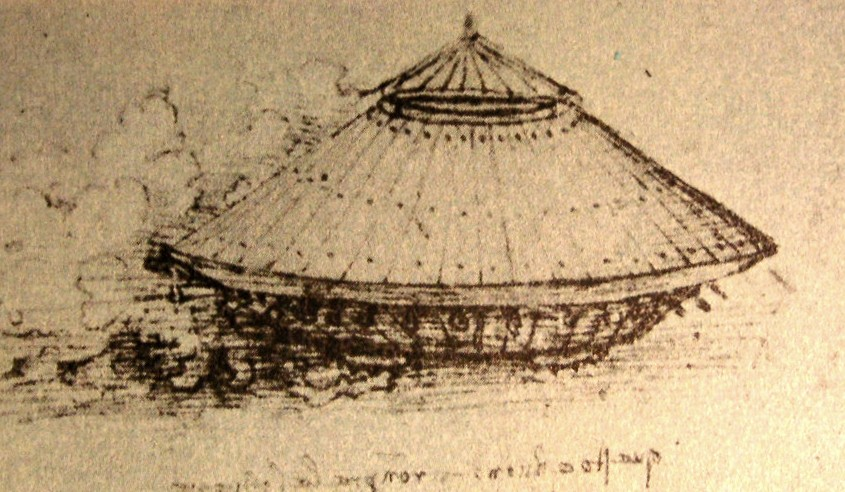
\includegraphics[scale=0.25]{imgs/Leonardo_tank.jpg}
 	\caption[Czołg Leonarda da Vinci]{\small{Szkic Leonarda da Vinci przedstawiający jego koncepcję czołgu.}\footnotemark}
	\label{czolg_leon}
    \end{center}
  \end{figure}
  \footnotetext{\emph{Czołg Leonarda da Vinci}, http://italoteka.blogspot.com,  (data dostępu 21.04.2015r.)}
Wiek XX niesie za sobą bardzo gwałtowny rozwój robotyki, który rozpoczął się w momencie skonstruowania w latach 40-tych pierwszego komputera. Ich rozwój był dodatkowo spotęgowany poprzez wybuch II wojny światowej i potrzebę łamania szyfrów dyplomatycznych.
W latach 50-tych wynaleziony został tranzystor, który aktualnie jest podstawowym elementem każdego urządzenia. Pozwolił on w znacznej mierze na zmniejszenie gabarytów komputerów (jednostek obliczeniowych), zmniejszenie zapotrzebowania na energię oraz wzrost mocy obliczeniowej co pozwoliło na konstrukcję autonomicznych robotów mobilnych.
Robotami mobilnymi nazywamy pojazdy, mogące zmieniać swoje położenie w przestrzeni. Dotyczy to nie tylko pojazdów jezdnych, ale także kroczących oraz latających. 
W 1956 r. ukończona została budowa elektrycznej wiewiórki\cite{robot_squee} (rysunek \ref{squee}), która posiadała dwa ,,zmysły": wzroku - zrealizowanego przy wykorzystaniu dwóch lamp fotoelektronowych oraz dotyku - dwóch krańcówek.  Napęd został zbudowany w oparciu o silniki elektryczne. Zwierzak, gdy zobaczył żołędzia (w tym przypadku jasno oświetlony punkt) kierował się w jego stronę, podnosił owoc przy pomocy ,,szufli" a następnie kierował się ,,do gniazda" - czyli miejsca, gdzie znajdowało się pulsacyjne źródło światła. Mimo ,iż realizowane zadanie jest bardzo proste to możemy mówić tutaj o pewnego rodzaju intelgencji ponieważ wiewiórka wykonywała pewną sekwencję ruchową bez interwencji człowieka ale w zależności od tego, co działo sie w jej otoczeniu.

  \begin{figure}[H]
    \begin{center}
      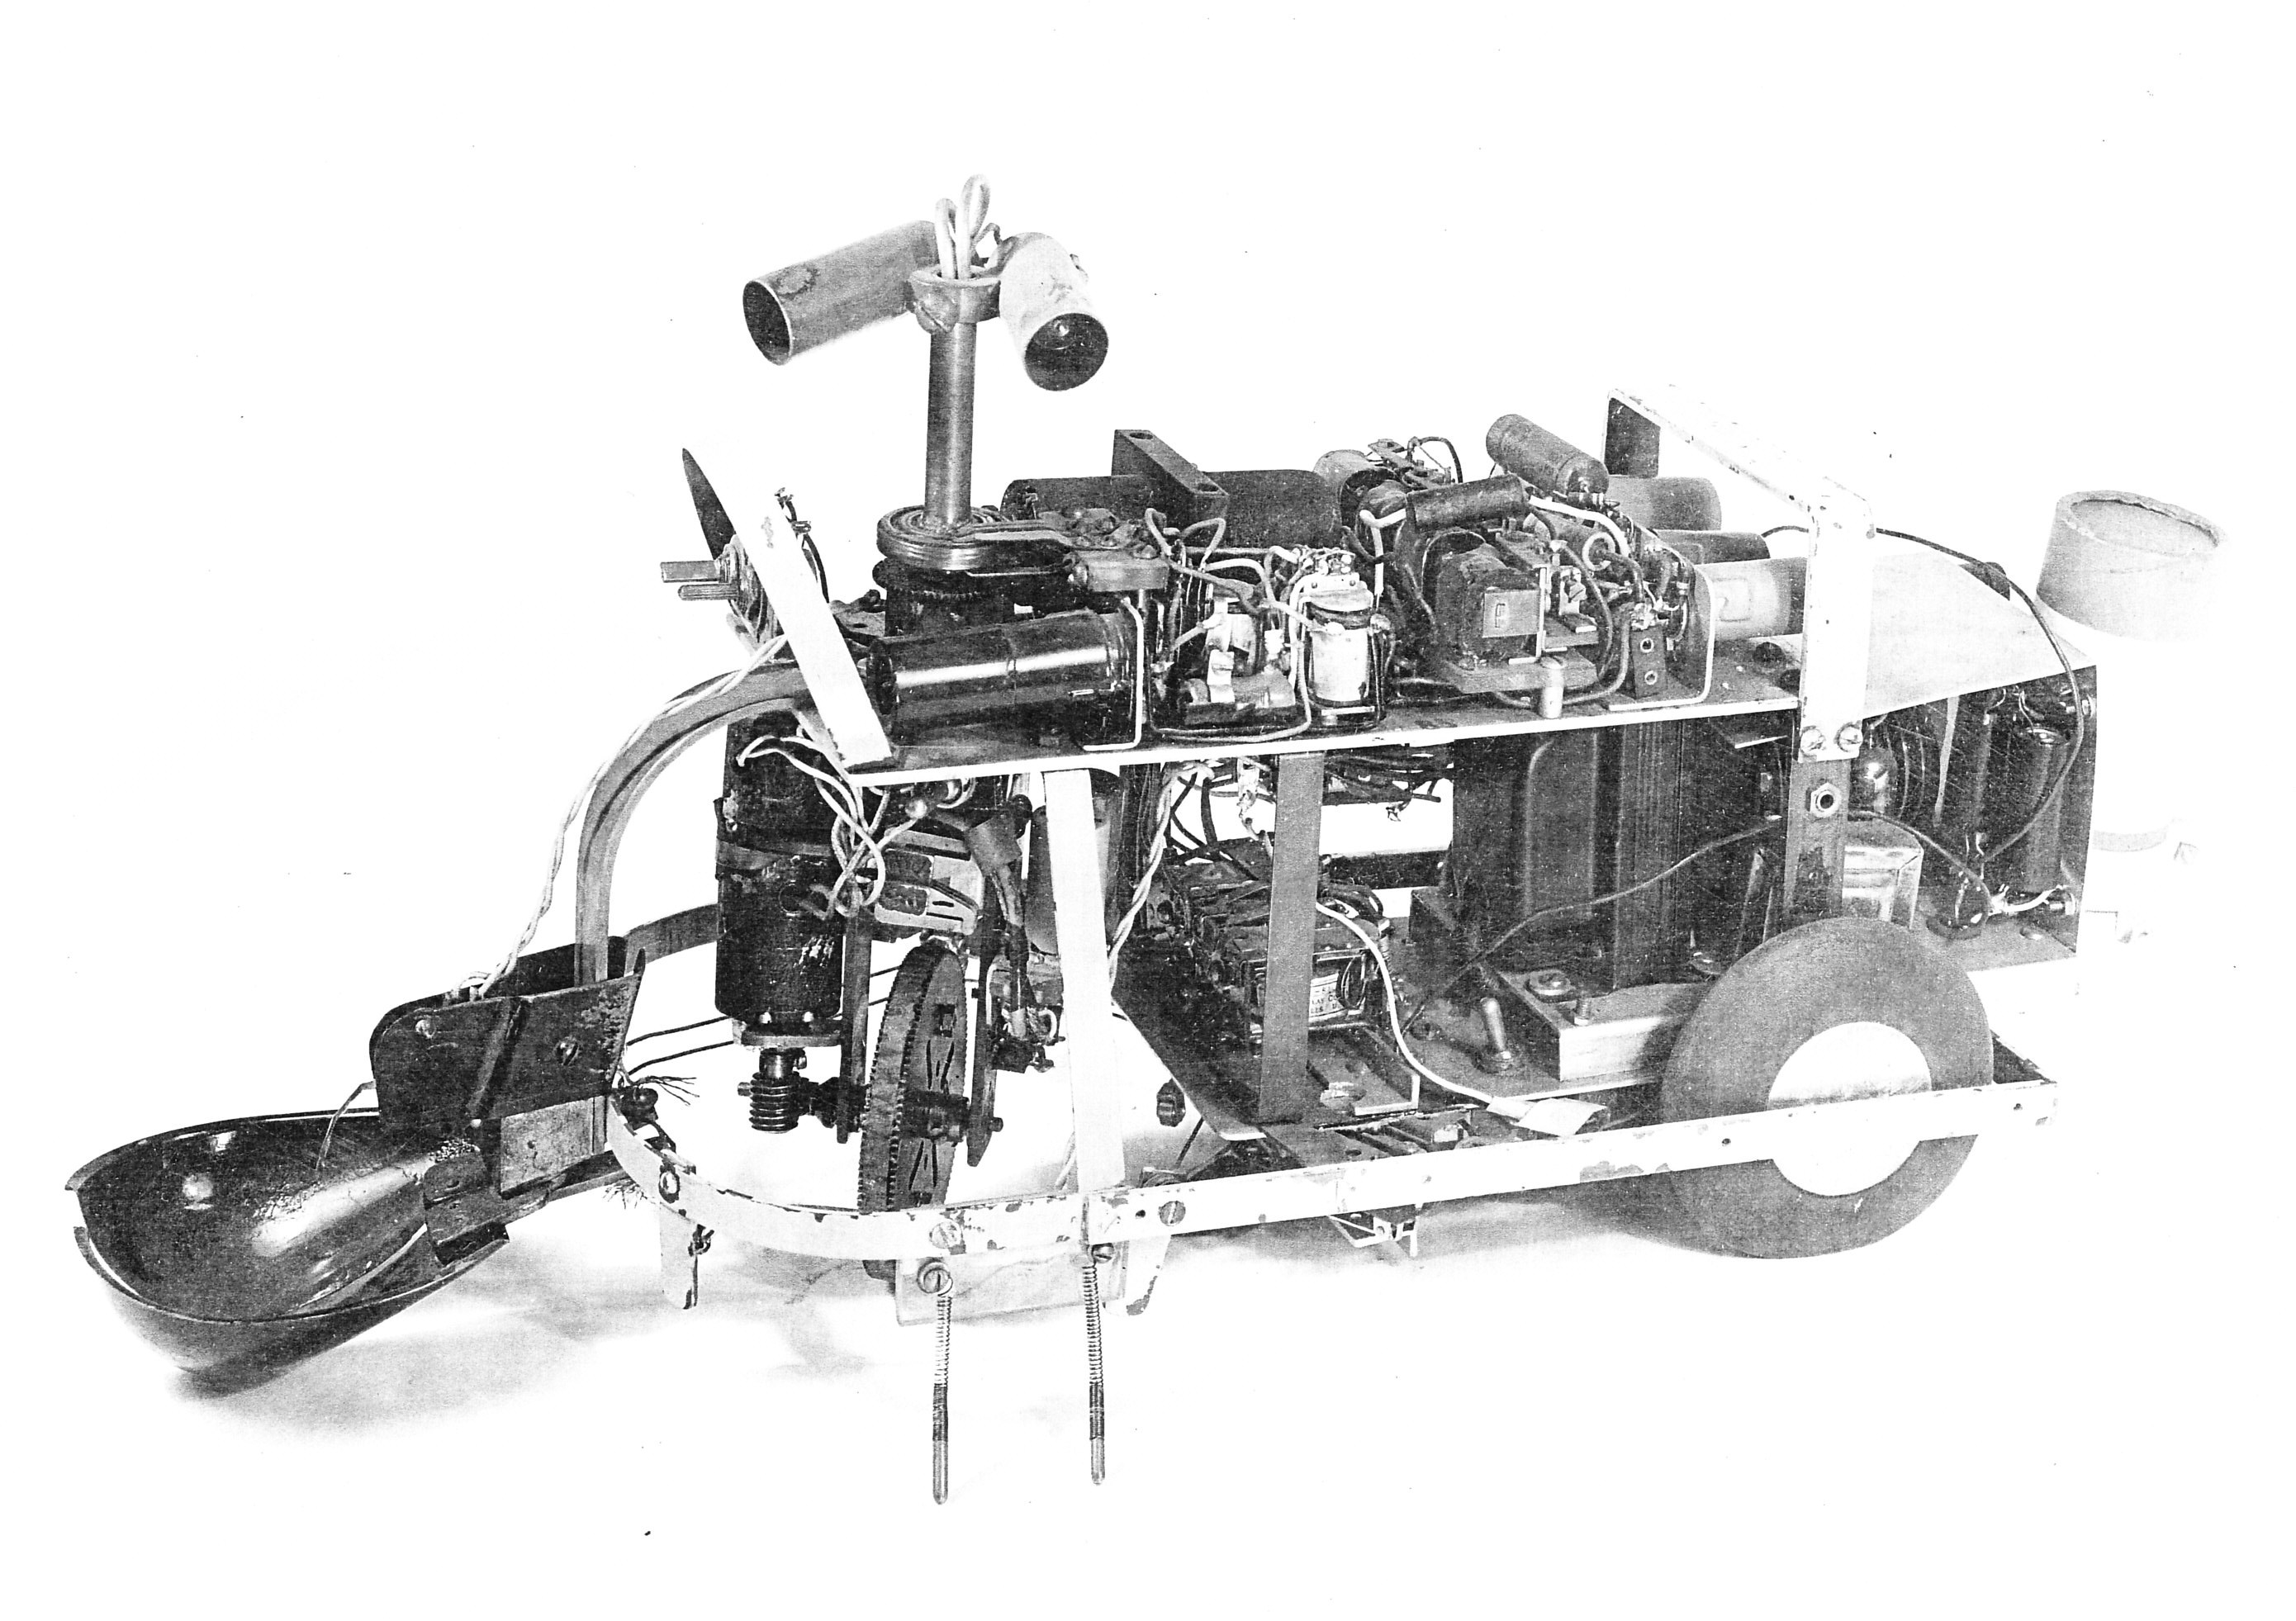
\includegraphics[scale=0.35]{imgs/Squee.jpg}
 \caption[Robot \textit{Squee}]{\small{Robot Squee zbudowany prze Jacka Koffa w 1959r.}\footnotemark}
        \label{squee}
    \end{center}
  \end{figure}
  \footnotetext{\emph{Robot Squee}, http://cyberneticzoo.com/,  (data dostępu 21.09.2015r.)}

Kolejne lata niosą za sobą coraz większą miniaturyzację wszelkich podzespów elektronicznych. Nie tylko zamykane są one w coraz mniejszych obudowach (pierwszy układ scalony - Jack St. Clair Kilby w 1958 r.) ale także charakteryzują się coraz wyższą sprawnością. Doprowadza to do tego, że pojazdy mobilne stają się obiektem zainteresowania służb specjalnych. W ten sposób w 1984 r. powstaje Prowler (rysunek \ref{state}) - pierwszy zdalnie sterowany robot o przeznaczeniu militarnym. Platforma ta mogła pełnić różne funkcje: od roli wsparcia - wyposażona w karabiny maszynowe, po funkcje rozpoznawcze - wyposażona w kamery.

  \begin{figure}[H]
    \begin{center}
      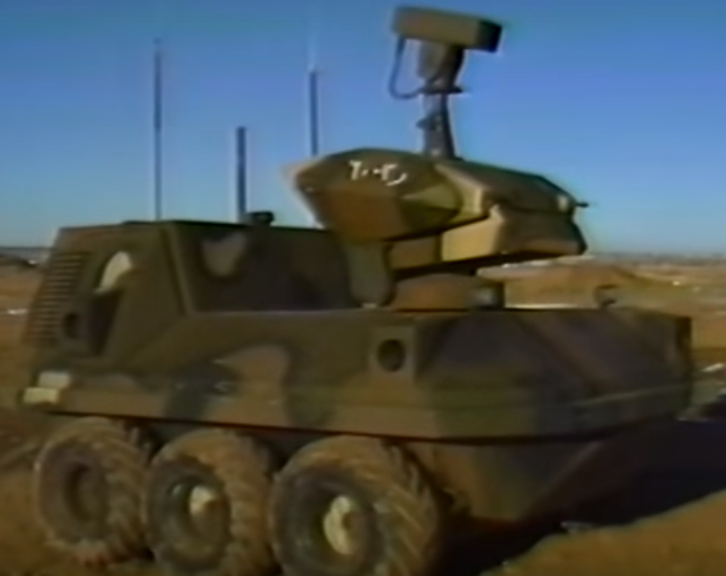
\includegraphics[scale=0.4]{imgs/state.png}
 \caption[Pojaz wojskowy \textit{Prowler}]{\small{Wojskowy robot mobilny Prowler .}\footnotemark}
        \label{state}
    \end{center}
  \end{figure}
  \footnotetext{\emph{Robot Defense Systems Prowler 1985}, https://youtube.com/,  (data dostępu 22.09.2015r.)}

Aktualnie najbardziej zaawansowanymi robotami mobilnymi są pojazdy wykorzystywane przez agencje kosmiczne do eksploracji kosmosu. Ich zaawansowana konstrukcja jest efektem bardzo rygorystycznych założeń jakie są im stawiane, tzn.: możliwie jak najmniejsze rozmiary, waga, wysoka mobilność oraz niezawodność, możliwość pracy w ciężkich, nieznanych warunkach środowiskowych. Na dodatek muszą one być zdolne do prowadzenia badań oraz zbierania próbek. Przykładem tej klasy robota może być marsjański łazik Curiosity Rover (rysunek \ref{lazik}).

  \begin{figure}[H]
    \begin{center}
      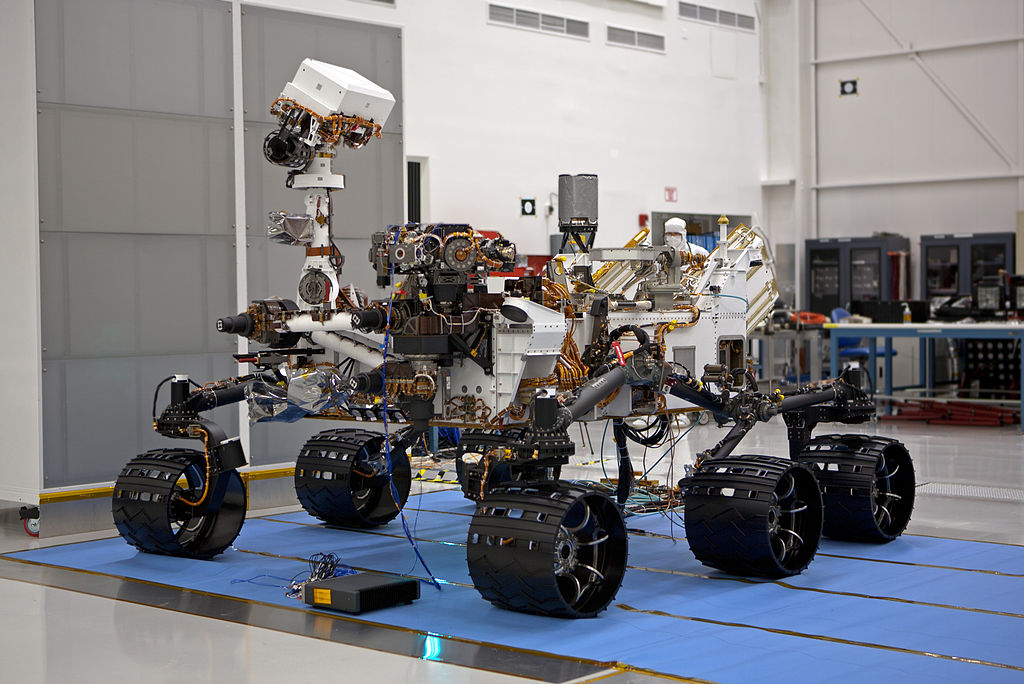
\includegraphics[scale=0.8]{imgs/curiosity.png}
 \caption[Łazik marsjański \textit{Curiosity}]{\small{Łazik marsjański Curiosity.}\footnotemark}
        \label{lazik}
    \end{center}
  \end{figure}
  \footnotetext{\emph{\textit{Curiosity}}, http://i.space.com/,  (data dostępu 22.09.2015r.)}

\section{Konstrukcja}
%w tym miejscu ja skupi� si� na om�wieniu budowy czo�gu, jakie� przekroje, mo�e szkice - przede wszystkim skupie si� na om�wieniu sterowania wie�yczk� no i nap�dem
\section{Przetwarzanie obrazu}
Obraz cyfrowy, w dalszej cz�ci pracy nazywany po prostu obrazem, jest graficzn� reprezentacj� tablicy, kt�r� mo�na tak�e przedstawi� za pomoc� funkcji:
\begin{equation}
\label{funkcja_obrazu}
    z = f(x,y), dla: x = 0, 1, 2, ..., N-1; y = 0, 1, 2, ..., M-1
\end{equation}
gdzie:\\
$N$ - szeroko�� obrazu,\\
$M$ - wysoko�� obrazu\\
$z$ - warto�� funkcji w punkcie.\\
W najprostszym przypadku obraz�w czarno-bia�ych warto�ci� wyra�ana przez t� funkcj� jest stopie� szaro�ci ka�dego piksela (tj. najmniejszej sk�adowej obrazu cyfrowego, charakteryzuj�cej si� jednolit� barw�). Obraz sk�ada si� wtedy z jednej, dwuwymiarowej tablicy o wymiarach $N$ na $M$.

W przypadku obraz�w kolorowych jednak do przedstawienia obrazu stosuje si� kilka takich funkcji. Najpopularniejszym sposobem przedstawiania kolor�w w grafice komputerowej jest model RGB. Skr�t ten tworz� pierwsze litery angielskich nazw kolor�w b�d�cych baz� w tym modelu: \textit{red} (czerwony), \textit{green} (zielony) oraz \textit{blue} (niebieski), kt�rych odpowiednia kombinacja umo�liwia uzyskanie ka�dego koloru. W przypadku wykorzystania tego modelu obraz zapisany jest jako trzy tablice, przechowuj�ce odpowiednio nat�enia kolor�w czerwonego, zielonego i niebieskiego.

Obrazy, na kt�rych b�d� wykonywane operacje na potrzeby tego projektu b�d� obrazami rejestrowanymi przez kamer� zamontowan� na robocie, a wi�c odzwierciedlaj�cymi rzeczywiste otoczenie. Rejestracja rzeczywistego obrazu na posta� cyfrow� polega na dyskretyzacji obrazu oraz kwantyzacji jasno�ci koloru\cite{Malina}. Dyskretyzacja obrazu rzeczywistego polega na pr�bkowaniu go w dw�ch wymiarach. W ka�dym polu tabeli, odpowiadaj�cej za jeden kolor, zapisywana jest warto�� nat�enia danego koloru dla wycinka obrazu rzeczywistego, kt�remu odpowiada adres danego pola. Rejestrowane nat�enie ka�dego z kolor�w jest warto�ci� ci�g�� i w celu zapisania jej w pami�ci komputera stosuje si� kwantyzacj�, tj. podzieleniu ca�ego zakresu jasno�ci na przedzia�y i przypisywaniu warto�ci rejestrowanej do jednego z tych przedzia��w. Wynik tej operacji jest najcz�ciej zapisywany na 8 bitach, a wi�c posiada warto�ci od 0 do 255 ($2^8$ daje 256 kombinacji). Pami�taj�c, �e tworzone s� trzy tablice, osobna dla ka�dego z kolor�w RGB, a wi�c dane ka�dego piksela zapisywane s� na $3 x 8 = 24$ bitach. Daje to kombinacj� $2^24 = 16777216$ kolor�w, czyli ilo�� przekraczaj�c� ju� mo�liwo�ci percepcji ludzkiego oka.

\textit{Celem sztucznego przetwarzania lub analizy obrazu jest takie automatyczne przetworzenie i przeanalizowanie obrazu obiekt�w lub ca�ego otoczenia systemu zautomatyzowanego, aby uzyska� u�yteczn� informacj� na temat interesuj�cych obiekt�w (...) lub na temat otoczenia, kt�re mo�e wp�ywa� (...) na sterowany automatycznie proces.}\cite{Tadeusiewicz}

Czytaj�c powy�sz� definicj� nale�y by� �wiadomym, �e obraz rzeczywistego otoczenia posiada olbrzymi� ilo�� informacji, w znacznej mierze nadmiarowych, nie maj�cych zwi�zku z poszukiwanymi informacjami. Analizowanie obraz�w dokonywane w ludzkim m�zgu jest dla cz�owieka czynno�ci� naturaln�, �wiczon� od chwili narodzin. Wydaje si� wi�c by� czym� prostym. W rzeczywisto�ci pr�ba powt�rzenia tych proces�w w spos�b sztuczny jest rzecz� niezwykle trudn� i z�o�on�. Ca�y proces wydobywania informacji obrazu mo�na podzieli� na trzy etapy: przetwarzanie, analiz� oraz rozpoznawanie.

Przetwarzanie obrazu jest to proces, charakteryzuj�cy si� tym, �e na jego wyj�ciu, tak samo jak na wej�ciu, znajduje si� obraz cyfrowy. Operacje te wykonuje si� w celu poprawy jako�ci samego obrazu, uwypukleniu jego cech. Typowymi operacjami nale��cymi do dziedziny przetwarzania obrazu s� np. r�nego rodzaju filtracje czy wyostrzanie kraw�dzi.

Kolejnym procesem jest analiza obrazu b�d�cego wynikiem przetwarzania. Polega ona na zastosowaniu algorytm�w, kt�rych celem jest wyodr�bnienie poszukiwanych danych ilo�ciowych i jako�ciowych. Na wyj�ciu otrzymuje si� wi�c nie pe�en obraz, z ca�� nadmiarowo�ci� danych, a jedynie informacje u�yteczne w danym procesie.

Uzyskane w powy�szy spos�b informacje wykorzystuje si� na ostatnim etapie, tj. w procesie rozpoznawania. \textit{(...) w zadaniu rozpoznawania chodzi o rozpoznawanie przynale�no�ci rozmaitego typu obiekt�w (lub zjawisk) do pewnych klas}\cite{Tadeusiewicz_flasinski}. Algorytm odpowiedzialny za te dzia�ania opiera si� wi�c o zbi�r cech, kt�rych warto�ci dla danego obrazu s� otrzymywane w procesach przetwarzania i analizy obrazu. Nast�pnie wykorzystuje posiadane ju� regu�y (np. zdobyte za pomoc� algorytmu ucz�cego) aby m�c w spos�b ostateczny scharakteryzowa� obraz wej�ciowy.

\begin{thebibliography}{9}
% Dodajemy bibliografi� do spisu tre�ci
\addcontentsline{toc}{chapter}{Bibliografia}
\bibitem{SJP}
\emph{S�ownik j�zyka polskiego}, http://sjp.pwn.pl/, (data dost�pu 20.10.2015 r.)

\bibitem{Czech}
\textsc{Leszek Rafi�ski, Aleksandra Bobcow, Andrzej Grono}: \emph{Roboty mobilne z autonomiczn� nawigacj� - stan obecny i perspektywy na najbli�sze lata}. Gda�sk, 2007 r.  

\bibitem{def_robota}
\emph{Teoria robotyki}, http://robotyka.com/, (data dost�pu 21.10.2015~r.)

\bibitem{prawa_robota}
\emph{Prawa robotyki i bunt robot�w}, http://kopernik.org.pl/, (data dost�pu 11.10.2015~r.)

\bibitem{da_vinci}
\textsc{Eugeniusz Olszewski}: \emph{Leonardo da Vinci jako prekursor nauk technicznych}, 1969~r.

\bibitem{robot_squee}
\emph{Squee: The Robot Squirrel}, http://computerhistory.org/, (data dost�pu 22.10.2015~r.)

\bibitem{wojna_pancerna}
\textsc{Tim Ripley}: \emph{Wojna pancerna. Strategia i taktyka}. Warszawa, 2008~r.

\bibitem{programy_rozwoju}
\textsc{Wojciech Zajler, Marek �. Grabania}: \emph{Perspektywiczne programy rozwoju pojazd�w g�sienicowych}. �Szybkobie�ne Pojazdy G�sienicowe�, nr 2, 2003~r.

\bibitem{czolg_przyszlosci}
\textsc{Marek D�browski}: \emph{Czo�g � obecnie i w przysz�o�ci}. �Szybkobie�ne Pojazdy G�sienicowe� nr 2, 2011~r.

\bibitem{kierunek_rozwoju}
\textsc{Wojciech Zajler, Marek �. Grabania}: \emph{Koncepcja modu�owego specjalnego pojazdu wielozadaniowego}. �Szybkobie�ne Pojazdy G�sienicowe� nr 1, 2004~r.

\bibitem{Redlarski}
\textsc{Grzegorz Redlarski, Andrzej Grono, Mariusz D�bkowski}: \emph{Perspektywy rozwoju robotyki}. Gda�sk, 2004~r.

\bibitem{Tadeusiewicz}
\textsc{Ryszard Tadeusiewicz, Przemys�aw Korohoda}: \emph{Komputerowa analiza i przetwarzanie obraz�w}. Krak�w 1997~r.

\bibitem{Malina}
\textsc{Witlod Malina, Maciej Smiatacz}: \emph{Cyfrowe przetwarzanie obraz�w}. Warszawa 2008~r.

\bibitem{Tadeusiewicz_flasinski}
\textsc{Ryszard Tadeusiewicz, Mariusz Flasi�ski}: \emph{Rozpoznawanie obraz�w}. Warszawa 1991~r.


\end{thebibliography}

\listoftables
\listoffigures
\end{document}
